% Exemple de fichier fonctionnnant avec la classe CAp2012.cls
% Base :  
%	Classe pf2010.cls adpatée de pf2003 par Jean CHarlet
%	Classe pf2003.cls adpatée de ic2001 par Jean CHarlet
%
% 	Classe ic2001.cls adpatée de EEGDRI3 par Jean CHarlet
%
% 	Classe EEGDRI3.cls adpatée de ic2000 par Jean CHarlet
%
% 	Classe IC'2000 (ic2000.cls) par Jean Charlet
%
% 	adaptée de la classe IC'99 (afia99.cls) développée par Fabien Torre

%\documentclass{CAp2012}
\documentclass[publibook-draft]{CAp2012}

\newcommand{\verbfichex}{CAp2012.\xspace}
\newcommand{\verbfichclass}{CAp2012.cls\xspace}
\newcommand{\verbfichbst}{CAp2012.bst\xspace}


%\usepackage[pdftex]{pstricks}

\usepackage{verbatim}
\usepackage{subfigure}
\usepackage[french]{babel}
\usepackage[utf8]{inputenc}
\usepackage[T1]{fontenc}

\usepackage{natbib}

\newtheorem{algorithm}{Algorithme}
\newtheorem{definition}{Définition}

%%%%%%%%%%%%%%%%%%%%%%%%%%%%%%%%%%%%%%%%%%%%%%%%%%%%%%%%%%%%%%%%%%%%%%%
% Titre court si le titre fait plus de 40 caractères
%%%%%%%%%%%%%%%%%%%%%%%%%%%%%%%%%%%%%%%%%%%%%%%%%%%%%%%%%%%%%%%%%%%%%%%

\shorttitle{Batch Inverse Reinforcement Learning}

\shortouvrage{CAp 2012}

% Titre, auteur, pas de date

\title{Batch Imitation via Inverse Reinforcement Learning Without Solving the Direct Problem}

\author{\fontsize{12}{12}\selectfont{Edouard Klein\inst{1}\inst{2}, Matthieu Geist\inst{1}, Olivier Pietquin\inst{1}\inst{3}}}

\institute{
Sup\'elec,\\
IMS Research group, France\\
\texttt{prenom.nom@supelec.fr}
\and
Equipe ABC,\\
LORIA-CNRS, France
\and
UMI 2958\\
GeorgiaTech-CNRS, France
}


\begin{document}
\maketitle


\begin{abstract}
  This paper addresses the problem of apprenticeship learning, that is learning control policies from demonstration by an expert. An efficient framework for it is inverse reinforcement learning  (IRL). Based on the assumption that the expert maximizes a utility  function, IRL aims at learning the underlying reward from example trajectories. Many IRL algorithms assume that the reward function is linearly parameterized and rely on some or all of the following elements : complete trajectories from the expert, a generative model for Monte-Carlo estimations, known transition probabilities and the ability to repeatedly solve the forward problem. In this paper we introduce a simple gradient ascent algorithm that lifts all these constraints. Relying on a temporal difference method for the estimation of the expert's {\it feature expectation} and a good set of features, our algorithm devise a reward function compatible with the expert's demonstrated behavior with a small computational and sample complexity.
  \motscles{Apprentissage par renforcement, Apprentissage par renforcement inverse, Processus Decisionnel de Markov}
\end{abstract}
\section{Introduction}
\begin{itemize}
\item Intérêt de l'Apprenticeship learning
\item Intérêt de l'IRL pour faire de l'apprenticeship learning
\item Rapide point sur les limitations des algos d'IRL actuels
\begin{itemize}
\item \cite{ng2000algorithms} : Probabilités de transitions devant être connues
\item \cite{abbeel2004apprenticeship} et toutes les approches résumées dans \cite{neu2009training}: Résolution du problème direct à chaque itération
\end{itemize}
\end{itemize}
\section{Background}
\label{back.sec}
\begin{itemize}
\item Introduction rapide, pour les notations, des MDPs, du RL et de l'IRL
\item Résumé plus détaillé que précédemment des approches IRL actuelles
\item Introduction du travail de Ratliff
\end{itemize}
\section{Loss-augmented Feature Expectation Matching}
\begin{itemize}
\item Reprise de l'équation de Ratliff
\item Reprise de l'explication sur l'approximation de $Q$ de la section \ref{back.sec}.
\item Dérivation de l'algo à partir de ces deux éléments
\item Pseudo-code
\end{itemize}
\section{Experimental results}
\subsection{GridWorld}
\begin{itemize}
\item Description du setting (GridWorld, expert, nombre de trajectoires, etc.)
\item Description des réglages de LAFEM (fonction $l$ notamment, calcul exact de $\mu_E$)
\item Présentation des résultats (pas grand chose à dire)
\end{itemize}
\begin{figure}
\begin{minipage}[t]{.4\linewidth}
    \begin{center}
       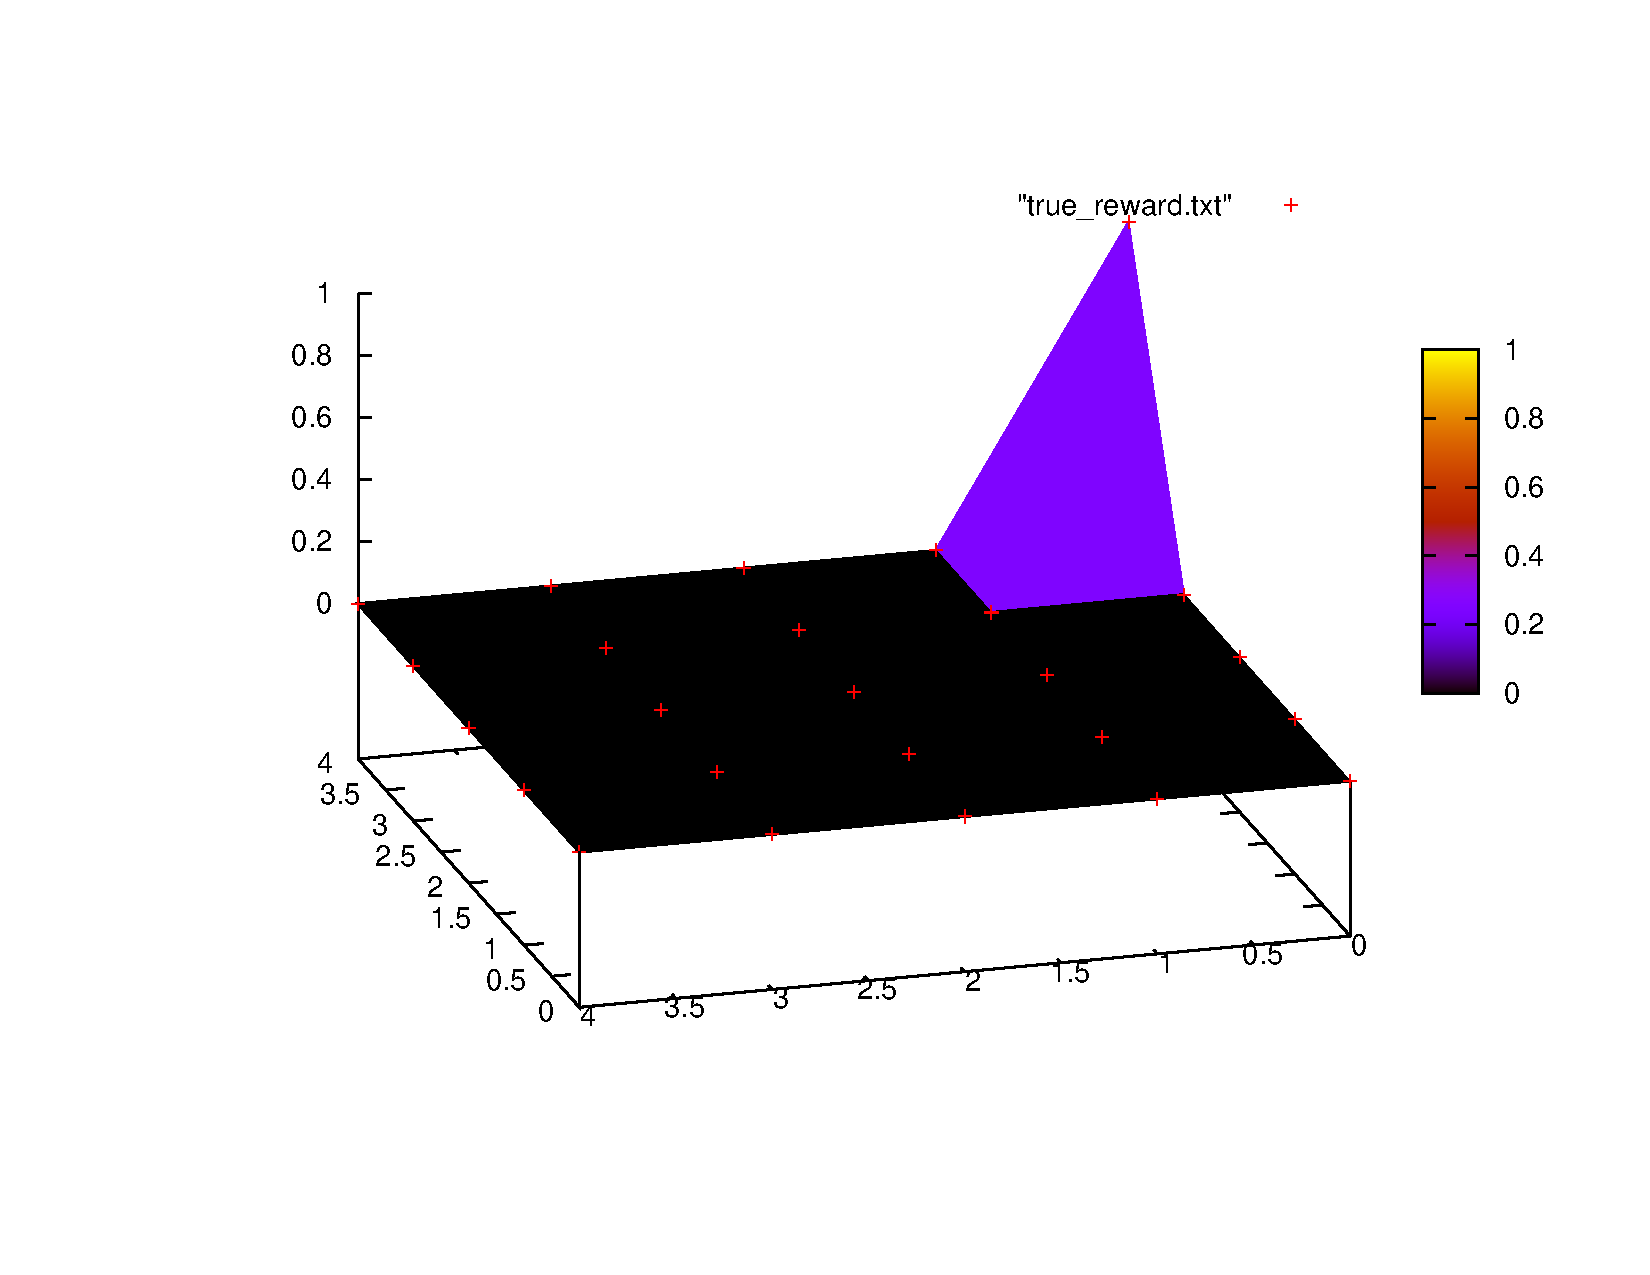
\includegraphics[width=\textwidth]{../GridWorld/true_reward.pdf}
       \caption{Expert's reward}
       \label{nbabo}
    \end{center}
\end{minipage}
\hfill
\begin{minipage}[t]{.4\linewidth}
    \begin{center}
       \includegraphics[width=\textwidth]{../GridWorld/retrieved_reward.pdf}
       \caption{Reward found by LAFEM}
       \label{croissnbabo}
    \end{center}
\end{minipage}\\
\begin{minipage}[t]{.4\linewidth}
    \begin{center}
       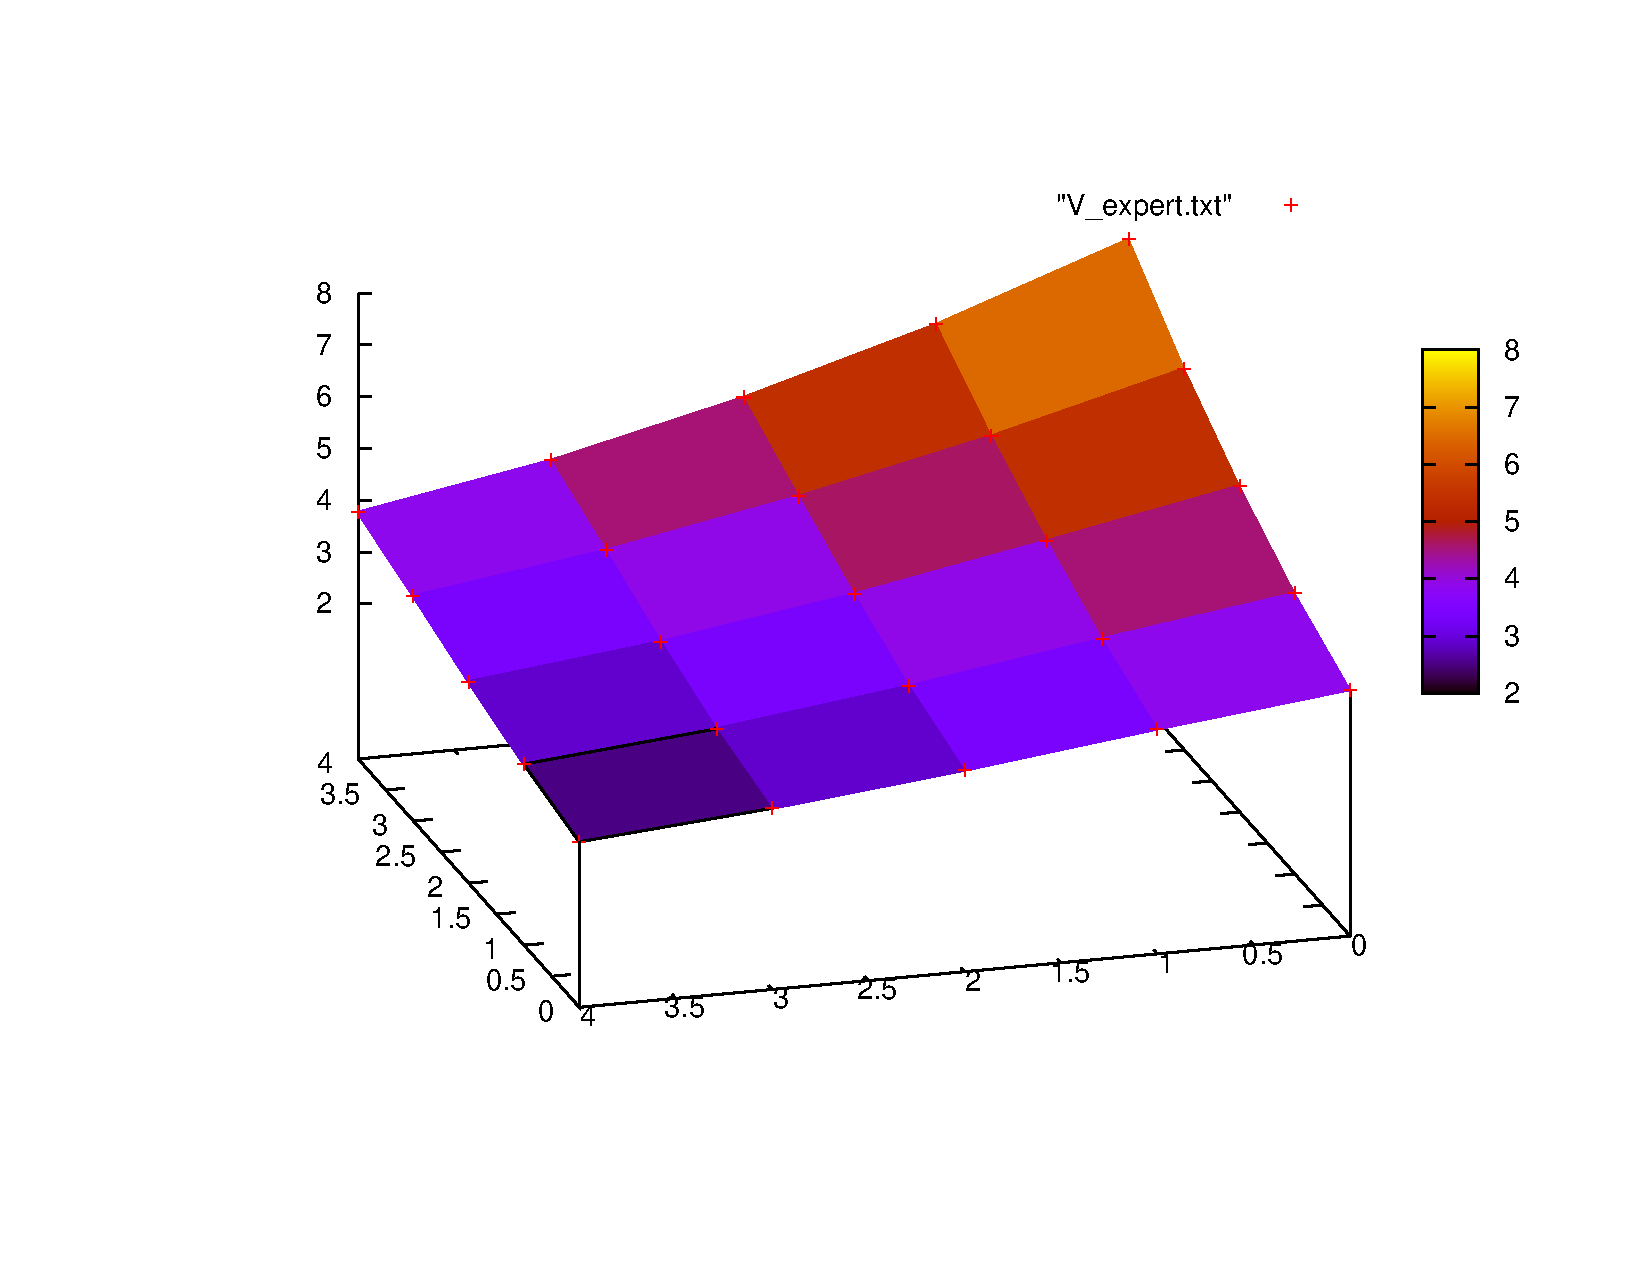
\includegraphics[width=\textwidth]{../GridWorld/V_expert.pdf}
       \caption{Expert's reward}
       \label{nbabo}
    \end{center}
\end{minipage}
\hfill
\begin{minipage}[t]{.4\linewidth}
    \begin{center}
       \includegraphics[width=\textwidth]{../GridWorld/V_agent.pdf}
       \caption{Agent's value function}
       \label{croissnbabo}
    \end{center}
\end{minipage}\\

\end{figure}

\subsection{Inverted Pendulum}
\begin{itemize}
\item Présentation du setting (Le pendule, l'expert)
\item Réglages de LAFEM (Préciser l'utilisation de LSTD$\mu$)
\item Présentation des résultats
\item Discussion sur la variabilité de la récompense
\item Présentation des performances statistiques (expérience pas encore effectuée)/ Etude de la complexité en échantillons 
\end{itemize}
\section{Conclusion and future work}
\begin{itemize}
\item On enlève les contraintes du domaine d'un seul coup, 
\item Il ne reste que la sélection ou détection de features, mais ce n'est pas hors de portée
\item Dans la même veine, il reste la résolution du problème direct une fois la récompense obtenue, il faut peut-être creuser du côté du reward shaping
\item Faible complexité computationnelle
\item Faible complexité en échantillons
\item Il reste des tests à faire sur le Highway driving (Pour ICML ?) et sur des expériences dans la vraie vie (bras robot ?)
\end{itemize}
%
% Bibliographie
%
\bibliography{../../Biblio/Biblio}

\end{document}

